\subsection{Algorithm Derivation Details} \label{sec:derivation}

The full optimization problem we solve, given the previous off-policy advantage estimate $A^{\pi_k}$ and buffer distribution $\pi_\beta$, is given below:
\begin{align}
    \pinew = \; \argmax_{\pi \in \Pi} \; & \E_{\at \sim \pi(\cdot|\st)}[A^{\pi_k}(\st, \at)] \\
    \text{s.t.} \; & \KL(\pi(\cdot|\st)||\pi_\buffer(\cdot|\st)) \leq \epsilon \\
    & \int_\at \pi(\at|\st) d\at = 1.
\end{align}
Our derivation follows~\citet{peters2010reps} and~\citet{peng2019awr}. The analytic solution for the constrained optimization problem above can be obtained by enforcing the KKT conditions. The Lagrangian is:
\begin{align}
    \mathcal{L}(\pi, \lagrangeawr, \alpha) = & \E_{\at \sim \pi(\cdot|\st)}[A^{\pi_k}(\st, \at)] \\ & + \lagrangeawr(\epsilon - \KL(\pi(\cdot|\st)||\piold(\cdot|\st))) \\ & + \alpha (1 - \int_\at \pi(\at|\st) d\at).
\end{align}
Differentiating with respect to $\pi$ gives:
\begin{align}
    \frac{\partial \mathcal{L}}{\partial \pi} = A^{\pi_k}(\st, \at) - \lagrangeawr \log \pi_\beta(\at|\st) + \lagrangeawr \log \pi(\at|\st) + \lagrangeawr - \alpha.
\end{align}
Setting $\frac{\partial \mathcal{L}}{\partial \pi}$ to zero and solving for $\pi$ gives the closed form solution to this problem:
\begin{align}
    \label{eqn:closedform}
    \pi^*(\at|\st) = \frac{1}{Z(\st)} \pi_\buffer(\at|\st)\exp\left(\frac{1}{\lagrangeawr} A^{\pi_k}(\st, \at)\right),
\end{align}
Next, we project the solution into the space of parametric policies. For a policy $\pi_\theta$ with parameters $\theta$, this can be done by minimizing the KL divergence of $\pi_{\theta}$ from the optimal non-parametric solution $\pi^*$ under the data distribution $\rho_{\pi_\buffer}(\st)$: 
\begin{align}
    & \argmin_\theta \; \Ex_{\rho_{\pi_\buffer}(\st) } \left[\KL(\pi^*(\cdot|\st)||\pi_\theta(\cdot|\st))\right] \\ = & 
    \argmin_\theta \; \Ex_{\rho_{\pi_\buffer}(\st)} \left[\Ex_{\pi^*(\cdot|\st)}[-\log \pi_\theta(\cdot|\st)]\right]
\end{align}
Note that in the projection step, the parametric policy could be projected with either direction of KL divergence. However, choosing the reverse KL direction has a key advantage: it allows us to optimize $\theta$ as a maximum likelihood problem with an expectation over data $s, a \sim \buffer$, rather than sampling actions from the policy that may be out of distribution for the Q function. In our experiments we show that this decision is vital for stable off-policy learning.

Furthermore, assume discrete policies with a minimum probably density of $\pi_\theta \geq \alpha_\theta$. Then the upper bound:
\begin{align}
    \KL(\pi^*||\pi_\theta) \leq & \frac{2}{\alpha_\theta} \DTV(\pi^*, \pi_\theta)^2 \\
    \leq & \frac{1}{\alpha_\theta} \KL(\pi_\theta||\pi^*)
\end{align}
holds by the Pinsker's inequality, where $\DTV$ denotes the total variation distance between distributions. Thus minimizing the reverse KL also bounds the forward KL. Note that we can control the minimum $\alpha$ if desired by applying Laplace smoothing to the policy.

\subsection{Implementation Details} \label{sec:implementation}

We implement the algorithm building on top of twin soft actor-critic~\citep{haarnoja2018sac}, which incorporates the twin Q-function architecture from twin delayed deep deterministic policy gradient (TD3) from~\citet{fujimoto2018td3}. All off-policy algorithm comparisons (SAC, BRAC, MPO, ABM, BEAR) are implemented from the same skeleton. The base hyperparameters are given in Table~\ref{table:rl-hyperparams}. The policy update is replaced with:
\begin{align}
    \theta_{k+1} = \argmax_\theta \; & \; \Ex_{\st, \at \sim \buffer}
    \left[\log \pi_\theta(\at|\st) \frac{1}{Z(\st)}  \exp \left(\frac{1}{\lagrangeawr}A^{\pi_k}(\st, \at) \right)\right].
\end{align}

\begin{table}[h!]
% {\columnwidth}
\footnotesize
% \vspace{-0.5cm}
\begin{tabular}{c|c|c}
Env      & \shortstack{Use \\ $Z(\st)$} & \shortstack{Omit \\ $Z(\st)$} \\ \hline
pen      & 84\%      & 98\%    \\
door     & 0\%      & 95\%    \\
relocate & 0\%      & 54\%
\end{tabular}
\caption{Success rates after online fine-tuning (after 800K steps for pen, door and 4M steps for relocate) using AWAC with and without $Z(\st)$ weight. These results show that although we can estimate $Z(\st)$, weighting by $Z(\st)$ actually results in worse performance.}
\label{fig:z}
\end{table}

Similar to advantage weight regression~\citep{peng2019awr} and other prior work~\citep{neumann2008fqiawr, wang2018marwil, siegel2020abm},
%%SL.10.1: Fill in citations to as many prior papers that do this as possible!
we disregard the per-state normalizing constant $Z(\st) = \int_\at \pi_\theta(\at|\st) \exp \left(\frac{1}{\lagrangeawr}A^{\pi_k}(\st, \at)\right) d\at = \E_{\at \sim \pi_\theta(\cdot|\st)}[A^{\pi_k}(\st, \at)]$. We did experiment with estimating this expectation per batch element with $K=10$ samples,
%%SL.10.1: Fill this in
but found that this generally made performance worse, perhaps because errors in the estimation of $Z(\st)$ caused more harm than the benefit the method derived from estimating this value. We report success rate results for variants of our method with and without $Z(\st)$ estimation in Table~\ref{fig:z}.
%%SL.10.1: Make sure to report both!
%Explicitly estimating $Z(\st)$ is worse than normalizing over a batch as we do. This shows that, although it is possible to estimate Z(\st), including this estimate actually hurts performance, perhaps because of high variance of evaluating the advantage on out-of-distribution actions.

%% AVN TODO fill in prior work
While prior work~\citep{neumann2008fqiawr, wang2018marwil, peng2019awr} has generally ignored the omission of $Z(\st)$ without any specific justification, it is possible to bound this value both above and below using the Cauchy-Schwarz and reverse Cauchy-Schwarz (Polya-Szego) inequalities, as follows.
Let $f(\at) = \pi(\at|\st)$ and $g(\at) = \exp(A(\st, \at)/\lambda)$. Note $f(\at) > 0$ for stochastic policies and $g(\at) > 0$.
By Cauchy-Schwarz, $Z(s) = \int_\at f(\at) g(\at) d\at \leq \sqrt{\int_\at f(\at)^2 d\at \int_\at g(\at)^2 d\at} = C_1$. To apply Polya-Szego, let $m_f$ and $m_g$ be the minimum of $f$ and $g$ respectively and $M_f, M_g$ be the maximum. Then $Z(\st) \geq 2 (\sqrt{\frac{M_f M_g}{m_f m_g} + \frac{m_f m_g}{M_f M_g}})^{-1} C_1 = C_2$. We therefore have $C_1 \leq Z(\st) \leq C_2$, though the bounds are generally not tight.
%, the overall KL objective can be bounded by these constant factors as well.
%%SL: I don't believe the overall KL objective can be bounded, but I added some more discussion
%%SL.10.1: Can you actually work this out? Can you argue that the bound is non-trivial (e.g., at convergence?) or quantify the resulting regret?

A further, more intuitive argument for why omitting $Z(\st)$ may be harmless in practice comes from observing that this normalizing factor only affects the relative weight of different \emph{states} in the training objective, not different actions. The state distribution in $\beta$ already differs from the distribution over states that will be visited by $\pi_\theta$, and therefore preserving this state distribution is likely to be of limited utility to downstream policy performance. Indeed, we would expect that sufficiently expressive policies would be less affected by small to moderate variability in the state weights. On the other hand, inaccurate estimates of $Z(\st)$ may throw off the training objective by increasing variance, similar to the effect of degenerate importance weights.

% We found that explicitly computing $Z(s) = \int_\at \pi_\buffer(\at|\st)\exp(\frac{1}{\lagrangeawr} A^{\pi_k}(\st, \at)) d\at$ results in worse performance, so we ignore the effect of $Z(s)$ and empirically find that this results in strong performance both offline and online.

The Lagrange multiplier $\lagrangeawr$ is treated as a hyperparameter in our method. In this work we use $\lagrangeawr = 0.3$ for the manipulation environments and $\lagrangeawr = 1.0$ for the MuJoCo benchmark environments. One could adaptively learn $\lagrangeawr$ with a dual gradient descent procedure, but this would require access to $\pi_\beta$.

As rewards for the dextrous manipulation environments are non-positive, we clamp the Q value for these experiments to be at most zero. We find this stabilizes training slightly.

\begin{table}
    \centering
    \begin{tabular}{c|c}
    \hline
    \textbf{Hyper-parameter} & \textbf{Value} \\
    \hline
    Training Batches Per Timestep & $1$\\
    Exploration Noise & None (stochastic policy) \\
    RL Batch Size & $1024$ \\
    Discount Factor & $0.99$\\
    Reward Scaling & $1$\\
    Replay Buffer Size & $1000000$\\
    Number of pretraining steps & $25000$ \\
    Policy Hidden Sizes & $[256, 256, 256, 256]$\\
    Policy Hidden Activation & ReLU\\
    Policy Weight Decay & $10^{-4}$ \\
    Policy Learning Rate & $3 \times 10^{-4}$\\
    Q Hidden Sizes & $[256, 256, 256, 256]$\\
    Q Hidden Activation & ReLU\\
    Q Weight Decay & $0$ \\
    Q Learning Rate & $3 \times 10^{-4}$\\
    Target Network $\tau$ & $5\times10^{-3}$ \\
    \hline
    \end{tabular}
\caption{Hyper-parameters used for RL experiments.}
\label{table:rl-hyperparams}
\end{table}

\subsection{Environment-Specific Details} \label{sec:environment_impl}

We evaluate our method on three domains: dexterous manipulation environments, Sawyer manipulation environments, and MuJoCo benchmark environments. In the following sections we describe specific details.

\subsubsection{Dexterous Manipulation Environments}

These environments are modified from those proposed by~\citet{rajeswaran2018dextrous}.
% , and available in \href{https://github.com/anair13/mj_envs}{this repository}.

\paragraph{pen-binary-v0.} The task is to spin a pen into a given orientation. The action dimension is 24 and the observation dimension is 45. Let the position and orientation of the pen be denoted by $x_p$ and $x_o$ respectively, and the desired position and orientation be denoted by $d_p$ and $d_o$ respectively. The reward function is $r = \mathds{1}_{|x_p - d_p| \leq 0.075} \mathds{1}_{|x_o \cdot d_o| \leq 0.95}$ - 1.
In~\citet{rajeswaran2018dextrous}, the episode was terminated when the pen fell out of the hand; we did not include this early termination condition.

\paragraph{door-binary-v0.} The task is to open a door, which requires first twisting a latch. The action dimension is 28 and the observation dimension is 39. Let $d$ denote the angle of the door. The reward function is $r = \mathds{1}_{d > 1.4}$ - 1.

\paragraph{relocate-binary-v0.} The task is to relocate an object to a goal location. The action dimension is 30 and the observation dimension is 39. Let $x_p$ denote the object position and $d_p$ denote the desired position. The reward is $r = \mathds{1}_{|x_p - d_p| \leq 0.1}$ - 1.

\subsubsection{Sawyer Manipulation Environment}

\paragraph{SawyerPush-v0.} This environment is included in the \href{https://github.com/vitchyr/multiworld}{Multiworld} library. The task is to push a puck to a goal position in a 40cm x 20cm, and the reward function is the negative distance between the puck and goal position. When using this environment, we use hindsight experience replay for goal-conditioned reinforcement learning. The random dataset for prior data was collected by rolling out an Ornstein-Uhlenbeck process with $\theta = 0.15$ and $\sigma = 0.3$.

\subsubsection{Off-Policy Data Performance}

The performances of the expert data, behavior cloning (BC) on the expert data (1), and BC on the combined expert+BC data (2) are included in Table~\ref{fig:bc}. For Gym benchmarks we report average return, and expert data is collected by a trained SAC policy. For dextrous manipulation tasks we report the success rate, and the expert data consists of human demonstrations provided by~\citet{rajeswaran2018dextrous}.

\begin{table}[h!]
% [\columnwidth]
\footnotesize
\begin{tabular}{c|c|c|c}
Env         & Expert & BC (1) & BC (2) \\ \hline
cheetah & 9962   & 2507         & 4524      \\
walker      & 5062   & 2040         & 1701      \\
ant         & 5207   & 687          & 1704      \\
pen         & 1      & 0.73          & 0.76       \\
door        & 1      & 0.10          & 0.00       \\
relocate    & 1      & 0.02          & 0.01       \\
\end{tabular}
% \vspace{-0.5cm}
\caption{Performance of the off-policy data for each environment. BC (1) indicates BC on the expert data, while BC (2) indicates BC on the combined expert+BC data used as off-policy data for pretraining. }
\label{fig:bc}
% \vspace{-0.6cm}
\end{table}

\begin{figure}[H]
    %\begin{flushleft}
    %\begin{subfigure}[t]{0.5\textwidth}
    \begin{centering}
        \footnotesize
        % \raisebox{3cm}{
        \begin{tabular}{ l||l|l|l|l  }
            Name & $\hat{Q}$ & Policy Objective & $\hat{\pi}_\beta$? & Constraint \\
            \hline
            SAC    & $Q^\pi$   & $\KL(\pi_\theta||\bar{Q})$   & No   &  None            \\
            SAC + BC & $Q^\pi$   & Mixed   & No   &  None            \\
            BCQ    & $Q^\pi$   & $\KL(\pi_\theta||\bar{Q})$   & Yes   &  Support ($\ell^\infty$)  \\
            BEAR   & $Q^\pi$   & $\KL(\pi_\theta||\bar{Q})$   & Yes   &  Support (MMD)   \\
            AWR    & $Q^\beta$ & $\KL(\bar{Q}||\pi_\theta)$   & No   &  Implicit        \\
            MPO    & $Q^\pi$   & $\KL(\bar{Q}||\pi_\theta)$   & Yes$^*$   &  Prior   \\
            ABM-MPO    & $Q^\pi$   & $\KL(\bar{Q}||\pi_\theta)$   & Yes   &  Learned Prior   \\
            DAPG   & -         & $J(\pi_\theta)$   & No   &  None            \\
            BRAC   & $Q^\pi$   & $\KL(\pi_\theta||\bar{Q})$   & Yes   &  Explicit KL penalty   \\
            AWAC (Ours)   & $Q^\pi$   & $\KL(\bar{Q}||\pi_\theta)$  & No    &  Implicit
        \end{tabular}
        % }
    %\end{subfigure}
    \end{centering}
    % \hfill
    %\end{flushleft}
    
    \caption{Comparison of prior algorithms that can incorporate prior datasets. See section~\ref{sec:baseline_impl} for specific implementation details. We argue that avoiding estimating $\hat{\pi}_\beta$ (i.e., $\hat{\pi}_\beta$ is ``No'') is important when learning with complex datasets that include experience from multiple policies, as in the case of online fine-tuning, and maintaining a constraint of some sort is essential for offline training. At the same time, sample-efficient learning requires using $Q^\pi$ for the critic. Our algorithm is the only one that fulfills all of these requirements.}
    \label{fig:algo_table}
\end{figure}

\subsection{Baseline Implementation Details} \label{sec:baseline_impl}

We used public implementations of prior methods (DAPG, AWR) when available. We implemented the remaining algorithms in our framework, which also allows us to understand the effects of changing individual components of the method. In the section, we describe the implementation details. The full overview of algorithms is given in Figure~\ref{fig:algo_table}.

\textbf{Behavior Cloning (BC).}  This method learns a policy with supervised learning on demonstration data.

\textbf{Soft Actor Critic (SAC).} Using the soft actor critic algorithm from \citep{haarnoja2018sac}, we follow the exact same procedure as our method in order to incorporate prior data, initializing the policy with behavior cloning on demonstrations and adding all prior data to the replay buffer. 

\textbf{Behavior Regularized Actor Critic (BRAC).} We implement BRAC as described in \citep{wu2019brac} by adding policy regularization $\log(\pi_\beta(a|s))$ where $\pi_\beta$ is a behavior policy trained with supervised learning on the replay buffer. We add all prior data to the replay buffer before online training. 

\textbf{Advantage Weighted Regression (AWR).} Using the advantage weighted regression algorithm from \citep{peng2019awr}, we add all prior data to the replay buffer before online training. We use the implementation provided by \citet{peng2019awr}, with the key difference from our method being that AWR uses TD($\lambda$) on the replay buffer for policy evaluation.

\textbf{Monotonic Advantage Re-Weighted Imitation Learning (MARWIL).} Monotonic advantage re-weighted imitation learning was proposed by~\citet{wang2018marwil} for offline imitation learning. MARWIL was not demonstrated in online RL settings, but we evaluate it for offline pretraining followed by online fine-tuning as we do other offline algorithms. Although derived differently, MARWIL and AWR are similar algorithms and only differ in value estimation: MARWIL uses the on-policy single-path advantage estimate $A(s, a) = Q^{\pi_\beta}(s, a) - V^{\pi_\beta}(s)$ instead of TD($\lambda$) as in AWR. Thus, we implement MARWIL by modifying the implementation of AWR.

\textbf{Maximum a Posteriori Policy Optimization (MPO).} We evaluate the MPO algorithm presented by~\citet{we2018mpo}. Due to a public implementation being unavailable, we modify our algorithm to be as close to MPO as possible. In particular, we change the policy update in \METHOD to be: 
\begin{align}
    \theta_i & \longleftarrow \argmax_{\theta_i} \; \; \E_{s \sim \mathcal{D}, a \sim \pi(a|s)} \; \nonumber \\ 
    &\left[\log \pi_{\theta_i}(a|s) \exp(\frac{1}{\beta}Q^\piold(s, a))\right].
\end{align}
Note that in MPO, actions for the update are sampled from the policy and the Q-function is used instead of advantage for weights. We failed to see offline or online improvement with this implementation in most environments, so we omit this comparison in favor of ABM.

\textbf{Advantage-Weighted Behavior Model (ABM).} We evaluate ABM, the method developed in \citet{siegel2020abm}. As with MPO, we modify our method to implement ABM, as there is no public implementation of the method. ABM first trains an advantage model $\pi_{\theta_\text{abm}}(a|s)$:
\begin{align}
    \theta_\text{abm} &= \argmax_{\theta_i} \; \; \E_{\tau \sim \mathcal{D}} \nonumber \\ &\left[\sum_{t=1}^{|\tau|} \log \pi_{\theta_\text{abm}}(a_t|s_t)f(R(\tau_{t:N})-\hat{V}(s))\right].
\end{align}
where $f$ is an increasing non-negative function, chosen to be $f = 1_+$. In place of an advantage computed by empirical returns $R(\tau_{t:N})-\hat{V}(s)$ we use the advantage estimate computed per transition by the $Q$ value $Q(s, a)-V(s)$. This is favorable for running ABM online, as computing $R(\tau_{t:N})-\hat{V}(s)$ is similar to AWR, which shows slow online improvement. We then use the policy update: 
\begin{align}
    \theta_i & \longleftarrow \argmax_{\theta_i} \; \; \E_{s \sim \mathcal{D}, a \sim \pi_\text{abm}(a|s)} \nonumber \\
    &\left[\log \pi_{\theta_i}(a|s)  \exp\left(\frac{1}{\lagrangeawr}(Q^{\pi_i}(s, a)-V^{\pi_i}(s))\right)\right].
\end{align}
Additionally, for this method, actions for the update are sampled from a behavior policy trained to match the replay buffer and the value function is computed as $V^\pi(s) = Q^\pi(s, a)$ s.t. $a \sim \pi$.

\textbf{Demonstration Augmented Policy Gradient (DAPG).} We directly utilize the code provided in ~\citep{rajeswaran2018dextrous} to compare against our method. Since DAPG is an on-policy method, we only provide the demonstration data to the DAPG code to bootstrap the initial policy from.

\begin{figure*}[t]
    \centering
    \begin{subfigure}[b]{0.02\textwidth}
        \center
        \begin{turn}{90} 
            \footnotesize
            Average Return
        \end{turn}
        \vspace{1.5cm}
    \end{subfigure}
    \begin{subfigure}[b]{0.3\textwidth}
        \center
        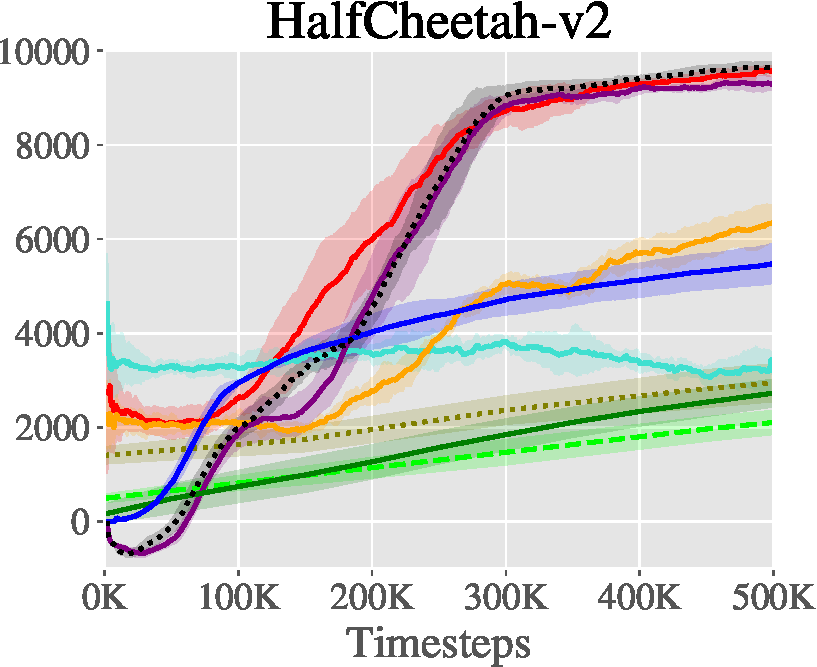
\includegraphics[width=\textwidth]{awac/figures/mujoco/hc-crop.pdf}
    \end{subfigure}
    \begin{subfigure}[b]{0.3\textwidth}
        \center
        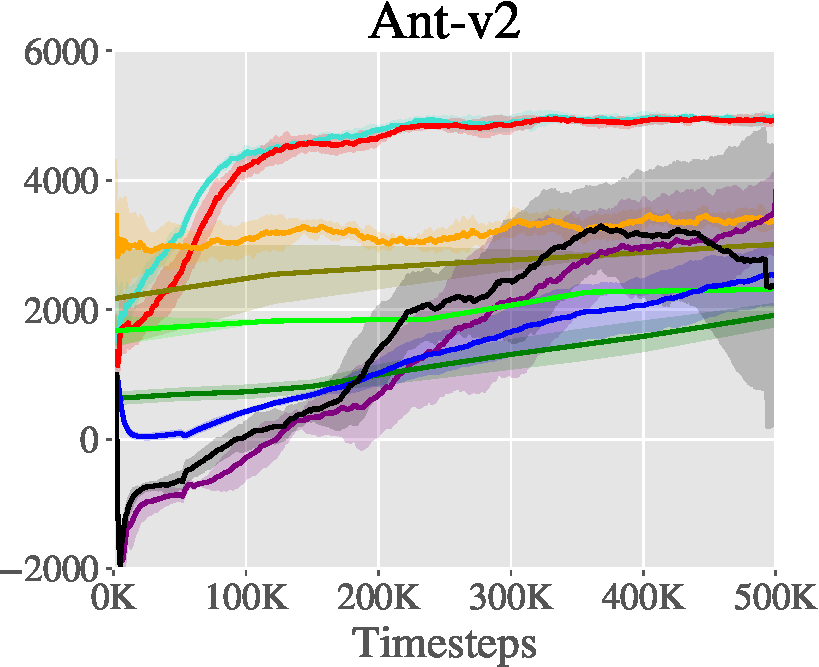
\includegraphics[width=\textwidth]{awac/figures/mujoco/ant-crop.pdf}
    \end{subfigure}
    \begin{subfigure}[b]{0.3\textwidth}
        \center
        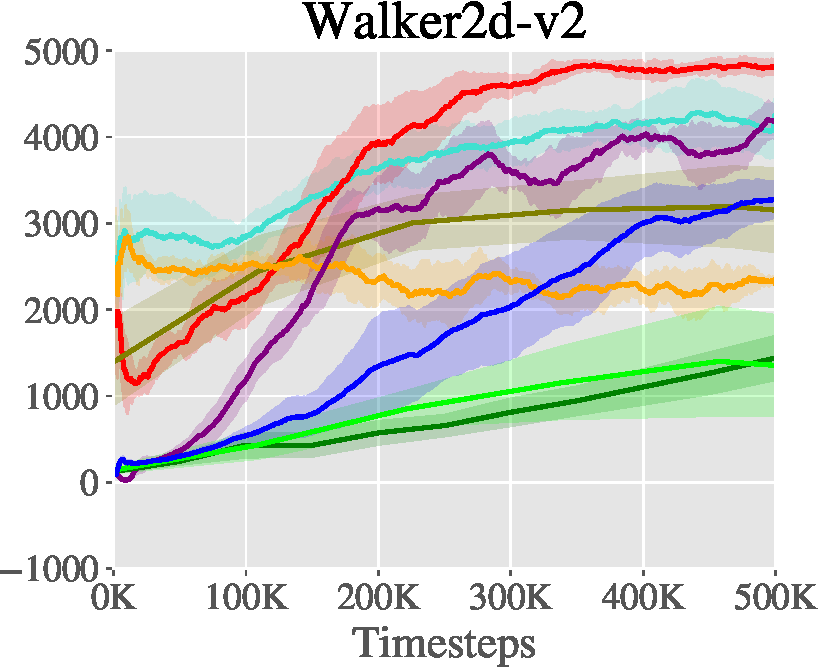
\includegraphics[width=\textwidth]{awac/figures/mujoco/walker-crop.pdf}
    \end{subfigure}
    
    \begin{subfigure}[b]{0.99\textwidth}
        \center
        % 
\includegraphics[width=1\textwidth]{awac/figures/mujoco/legend-crop.pdf}
        % 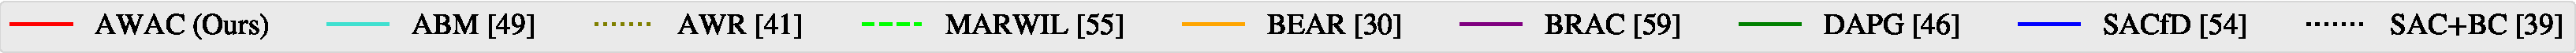
\includegraphics[width=1\textwidth]{awac/figures/mujoco/legend_ncol1-crop.pdf}
        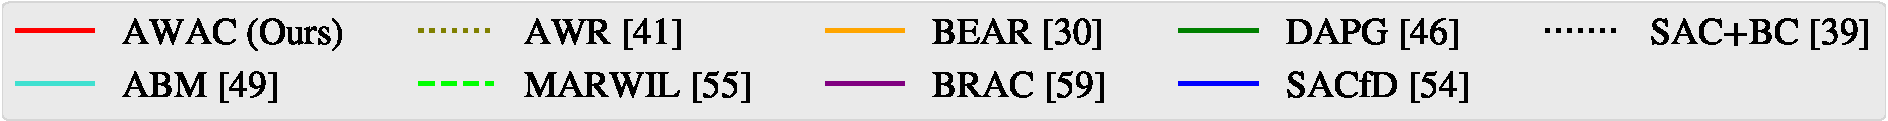
\includegraphics[width=0.6\textwidth]{awac/figures/mujoco/legend_ncol2-crop.pdf}
    \end{subfigure}
    \caption{
    % \footnotesize{
    Comparison of our method and prior methods on standard MuJoCo benchmark tasks. These tasks are much easier than the dexterous manipulation tasks, and allow us to better inspect the performance of methods in the setting of offline pretraining followed by online fine-tuning. SAC+BC and BRAC perform on par with our method on the HalfCheetah task, and ABM performs on par with our method on the Ant task, while our method outperforms all others on the Walker2D task. 
    Our method matches or exceeds the best prior method in all cases, whereas no other single prior method attains good performance on all of the tasks. }
    % }
    \label{fig:sim-learning-curves}
\end{figure*}

\textbf{Bootstrapping Error Accumulation Reduction (BEAR).} We utilize the implementation of BEAR provided in \href{https://github.com/vitchyr/rlkit}{rlkit}. We provide the demonstration and off-policy data to the method together. Since the original method only involved training offline, we modify the algorithm to include an online training phase. In general we found that the MMD constraint in the method was too conservative. As a result, in order to obtain the results displayed in our paper, we swept the MMD threshold value and chose the one with the best final performance after offline training with offline fine-tuning.

% \begin{wraptable}[12]{r}{2.1in}
% \footnotesize
% % \vspace{-1cm}
% \begin{tabular}{c|c|c|c}
% Env         & Expert & BC (1) & BC (2) \\ \hline
% cheetah & 9962   & 2507         & 4524      \\
% walker      & 5062   & 2040         & 1701      \\
% ant         & 5207   & 687          & 1704      \\
% pen         & 1      & 0.73          & 0.76       \\
% door        & 1      & 0.10          & 0.00       \\
% relocate    & 1      & 0.02          & 0.01       \\
% \end{tabular}
% \end{wraptable}

% \pagebreak

\subsection{Gym Benchmark Results From Prior Data}
\label{sec:gym}

In this section, we provide a comparative evaluation on MuJoCo benchmark tasks for analysis. These tasks are simpler, with dense rewards and relatively lower action and observation dimensionality. Thus, many prior methods can make good progress on these tasks. These experiments allow us to understand more precisely which design decisions are crucial. For each task, we collect 15 demonstration trajectories using a pre-trained expert on each task, and 100 trajectories of off-policy data by rolling out a behavioral cloned policy trained on the demonstrations. The same data is made available to all methods. The results are presented in Figure~\ref{fig:sim-learning-curves}. AWAC is consistently the best or on par with the best-performing method. No other single method consistently attains the best results -- on HalfCheetah, SAC + BC and BRAC are competitive, while on Ant-v2 ABM is competitive with AWAC.
We summarize the results according to the challenges in Section~\ref{sec:challenges}.

\textbf{Data efficiency.} The three methods that do not estimate $Q^\pi$ are DAPG~\citep{rajeswaran2018dextrous}, AWR~\citep{peng2019awr}, and MARWIL~\citep{wang2018marwil}. Across all three tasks, we see that these methods are somewhat worse offline than the best performing offline methods, and exhibit steady but very slow improvement during fine-tuning. In robotics, data efficiency is vital, so these algorithms are not good candidates for practical real-world applications.

\textbf{Bootstrap error in offline learning.} For SAC~\citep{haarnoja2018sac}, across all three tasks, we see that the offline performance at epoch 0 is generally poor. Due to the data in the replay buffer, SAC with prior data does learn faster than from scratch, but AWAC is faster to solve the tasks in general. SAC with additional data in the replay buffer is similar to the approach proposed by~\citet{vecerik17ddpgfd}. SAC+BC reproduces~\citet{nair2018demonstrations} but uses SAC instead of DDPG~\citep{lillicrap2015continuous} as the underlying RL algorithm. We find that these algorithms exhibit a characteristic dip at the start of learning. Although this dip is only present in the early part of the learning curve, a poor initial policy and lack of steady policy improvement can be a safety concern and a significant hindrance in real-world applications. Moreover, recall that in the more difficult dextrous manipulation tasks, these algorithms do not show any significant learning.

\textbf{Conservative online learning.} Finally, we consider  conservative offline algorithms: ABM~\citep{siegel2020abm}, BEAR~\citep{kumar19bear}, and BRAC~\citep{wu2019brac}. We found that BRAC performs similarly to SAC for working hyperparameters. BEAR trains well offline -- on Ant and Walker2d, BEAR significantly outperforms prior methods before online experience. However, online improvement is slow for BEAR and the final performance across all three tasks is much lower than AWAC. The closest in performance to our method is ABM, which is comparable on Ant-v2, but much slower on other domains. 

\pagebreak

\subsection{Extra Baseline Comparisons (CQL, AlgaeDICE)}

In this section, we add comparisons to constrained Q-learning (CQL)~\citep{kumar2020cql} and AlgaeDICE~\citep{nachum2019dualdice}. For CQL, we use the authors' implementation, modified for additionally online-finetuning instead of only offline training. For AlgaeDICE, we use the publicly available implementation, modified to load prior data and perform 25K pretraining steps before online RL. The results are presented in Figure~\ref{fig:cql-dice}.

\begin{figure}[H]
    \centering
    \begin{subfigure}[b]{0.49\textwidth}
        \center
        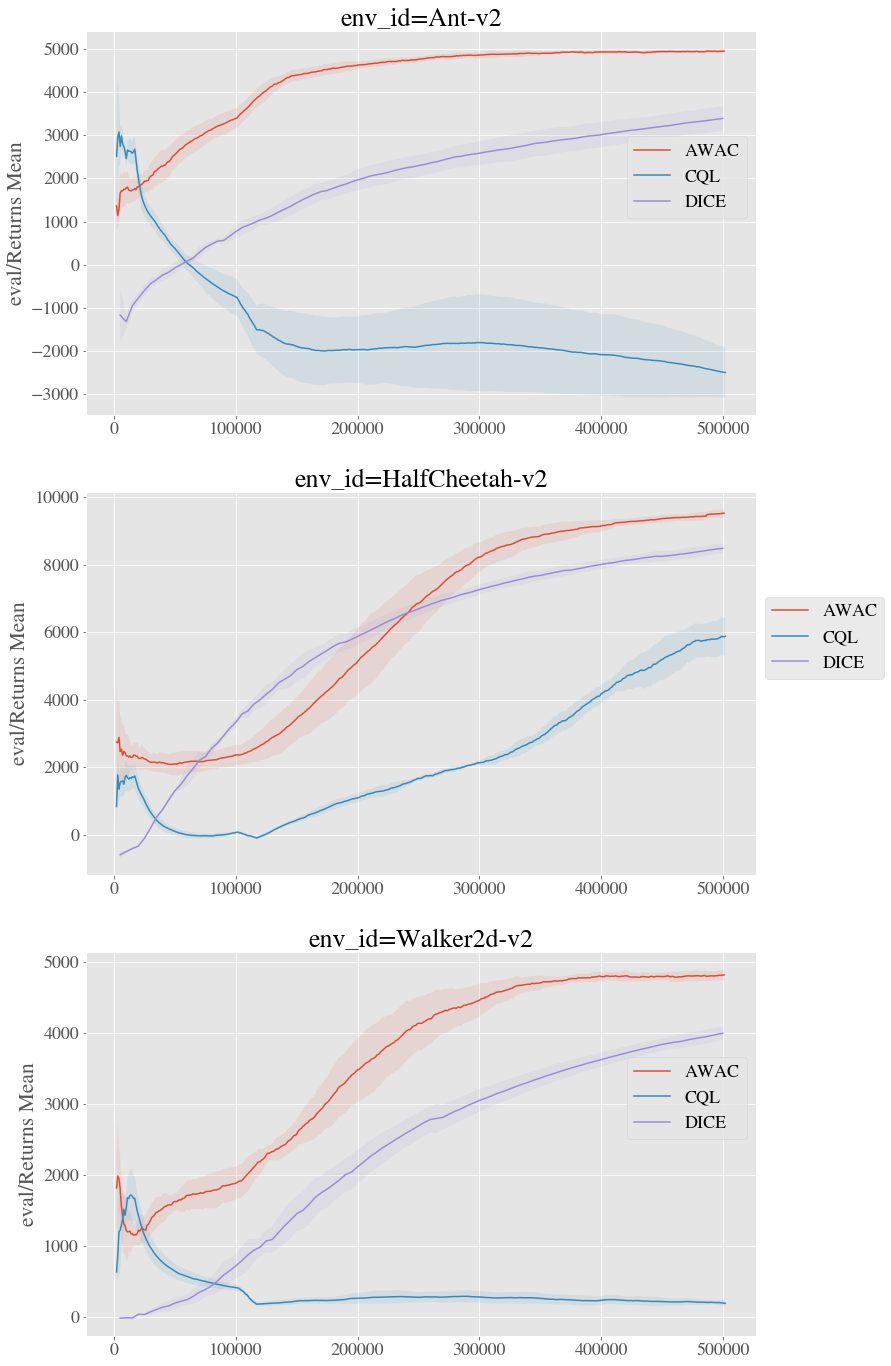
\includegraphics[width=\textwidth]{awac/figures/iclrrebuttal/d4rl_mujoco_comparisons.png}
    \end{subfigure}
    \begin{subfigure}[b]{0.49\textwidth}
        \center
        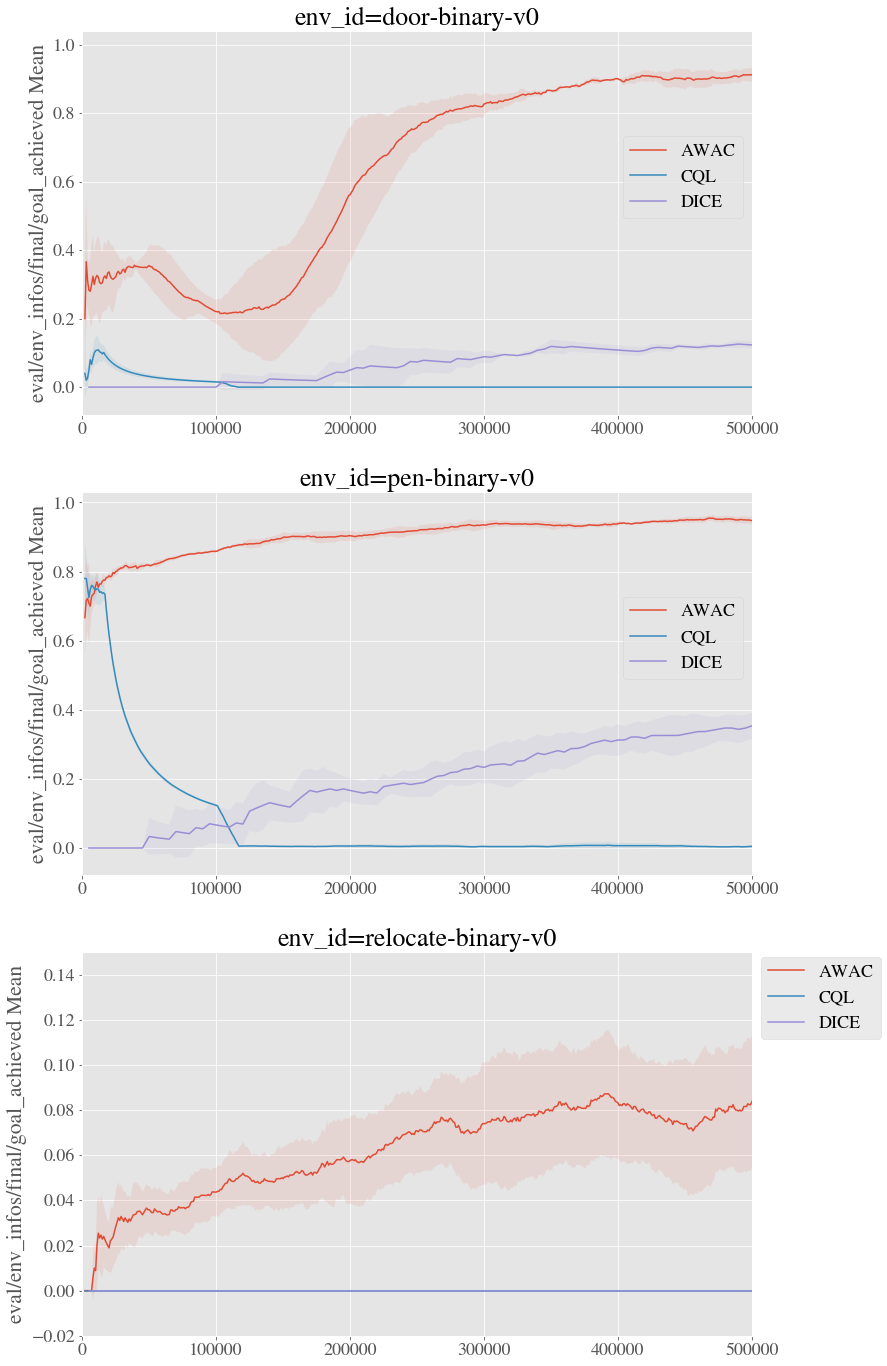
\includegraphics[width=\textwidth]{awac/figures/iclrrebuttal/d4rl_hand_comparisons.png}
    \end{subfigure}
    \caption{Comparison of our method (AWAC) with CQL and AlgaeDICE. CQL and AWAC perform similarly offline, but CQL does not improve when fine-tuning online. AlgaeDICE does not perform well for offline pretraining. }
    \label{fig:cql-dice}
\end{figure}

% \pagebreak

\subsection{Online Fine-Tuning From D4RL}

In this experiment, we evaluate the performance of varied data quality (random, medium, medium-expert, and expert) datasets included in D4RL~\citep{fu2020d4rl}, a dataset intended for offline RL. The results are obtained by first by training offline and then fine-tuning online on each setting for 500,000 additional steps. The performance of BEAR~\citep{kumar19bear} is attached as reference. We attempted to fine-tune BEAR online using the same protocol as AWAC but the performance did not improve and often decreased; thus we report the offline performance. All performances are scaled to 0 to 100, where 0 is the average returns of a random policy and 100 is the average returns of an expert policy (obtained by training online with SAC), as is standard for D4RL.

The results are presented in Figure~\ref{fig:d4rl_comparison}. First, we observe that AWAC (offline) is competitive with BEAR, a commonly used offline RL algorithm. Then, AWAC is able to make progress in solving the tasks with online fine-tuning, even when initialized from random data or “medium” quality data, as shown by the performance of AWAC (online). In almost all settings, AWAC (online) is the best performing or tied with BEAR. In four of the six lower quality (random or medium) data settings, AWAC (online) is significantly better than BEAR; it is reasonable that AWAC excels in the lower-quality data regime because there is more room for online improvement, while both offline RL methods often start at high performance when initialized from higher-quality data.

\begin{figure}[H]
% \begin{table}[]
\begin{tabular}{lllll}
 &    & \begin{tabular}[c]{@{}l@{}}AWAC\\ (offline)\end{tabular} & \begin{tabular}[c]{@{}l@{}}AWAC\\ (online)\end{tabular} & BEAR \\
HalfCheetah & random & 2.2 & \textbf{52.9}  & 25.5 \\
 & medium & 37.4 & 41.1 & 38.6 \\
 & medium-expert & 36.8 & 41.0 & \textbf{51.7} \\
 & expert & 78.5 & 105.6 & 108.2         \\
Hopper      & random & 9.6 & \textbf{62.8} & 9.5 \\
 & medium & 72.0 & \textbf{91.0} & 47.6 \\
 & medium-expert & 80.9 & \textbf{111.9} & 4.0 \\
 & expert  & 85.2 & 111.8 & 110.3 \\
Walker2D  & random & 5.1 & 11.7 & 6.7 \\
 & medium & 30.1 & \textbf{79.1} & 33.2 \\
 & medium-expert & 42.7 & \textbf{78.3} & 10.8 \\
 & expert & 57.0 & 103.0 & 106.1        
\end{tabular}
% \end{table}
\caption{Comparison of our method (AWAC) fine-tuning on varying data quality datasets in  D4RL~\citep{fu2020d4rl}. AWAC is able to improve its offline performance by further fine-tuning online. }
\label{fig:d4rl_comparison}
\end{figure}

\begin{figure*}[t]
    \centering
    \begin{subfigure}[b]{0.32\textwidth}
        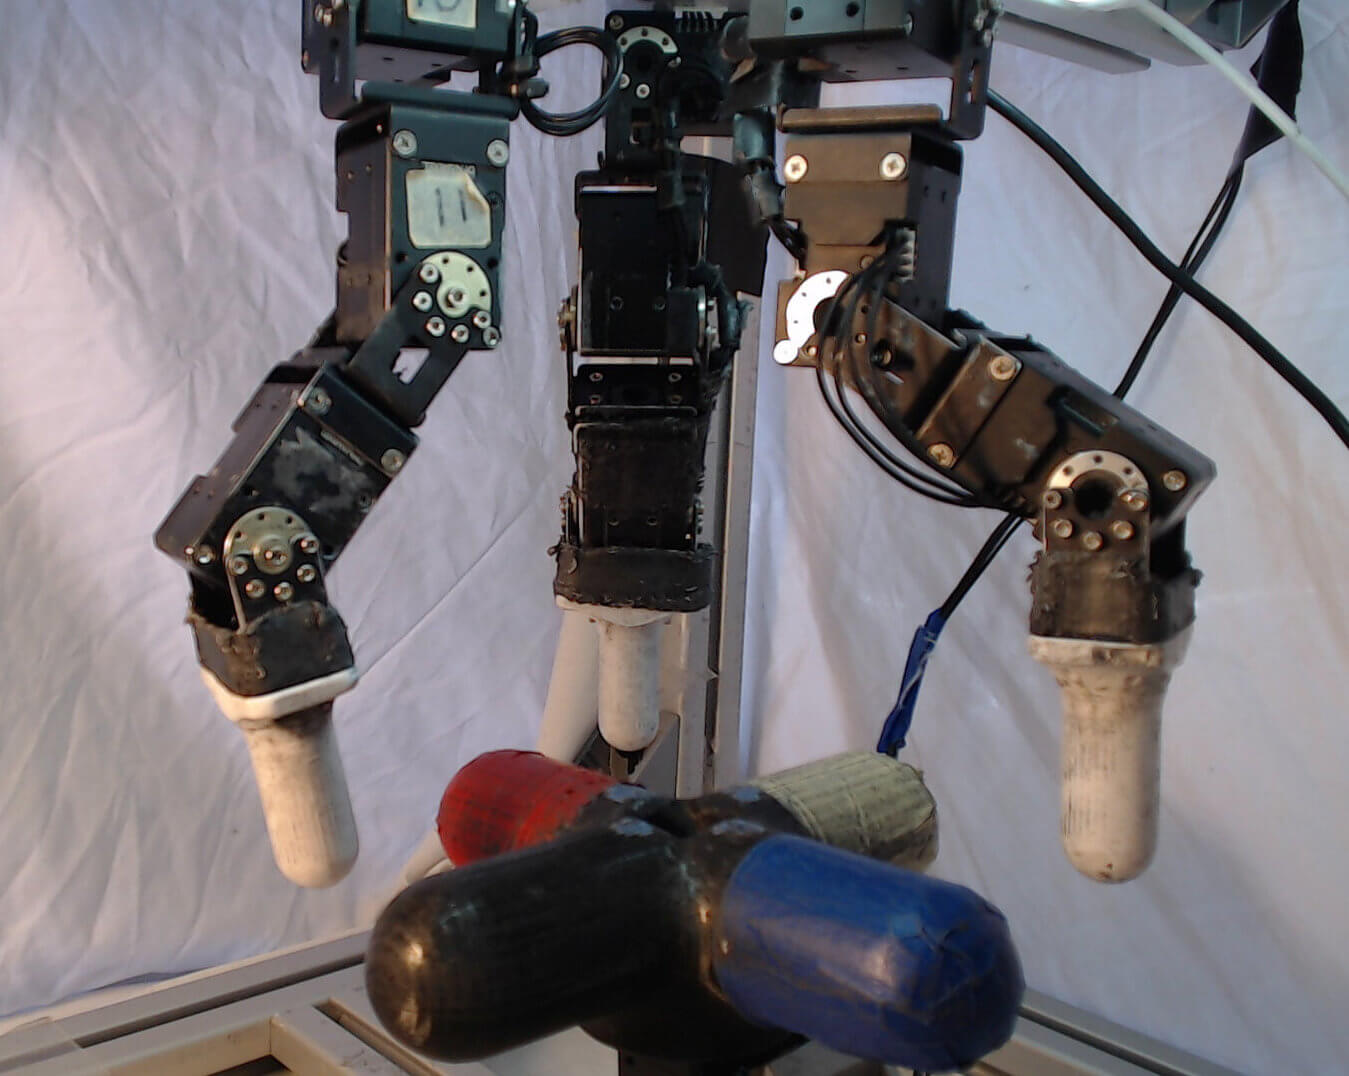
\includegraphics[height=0.6\textwidth]{awac/figures/robot/dclaw_new.jpg}
    \end{subfigure}
    \begin{subfigure}[b]{0.32\textwidth}
        \center
        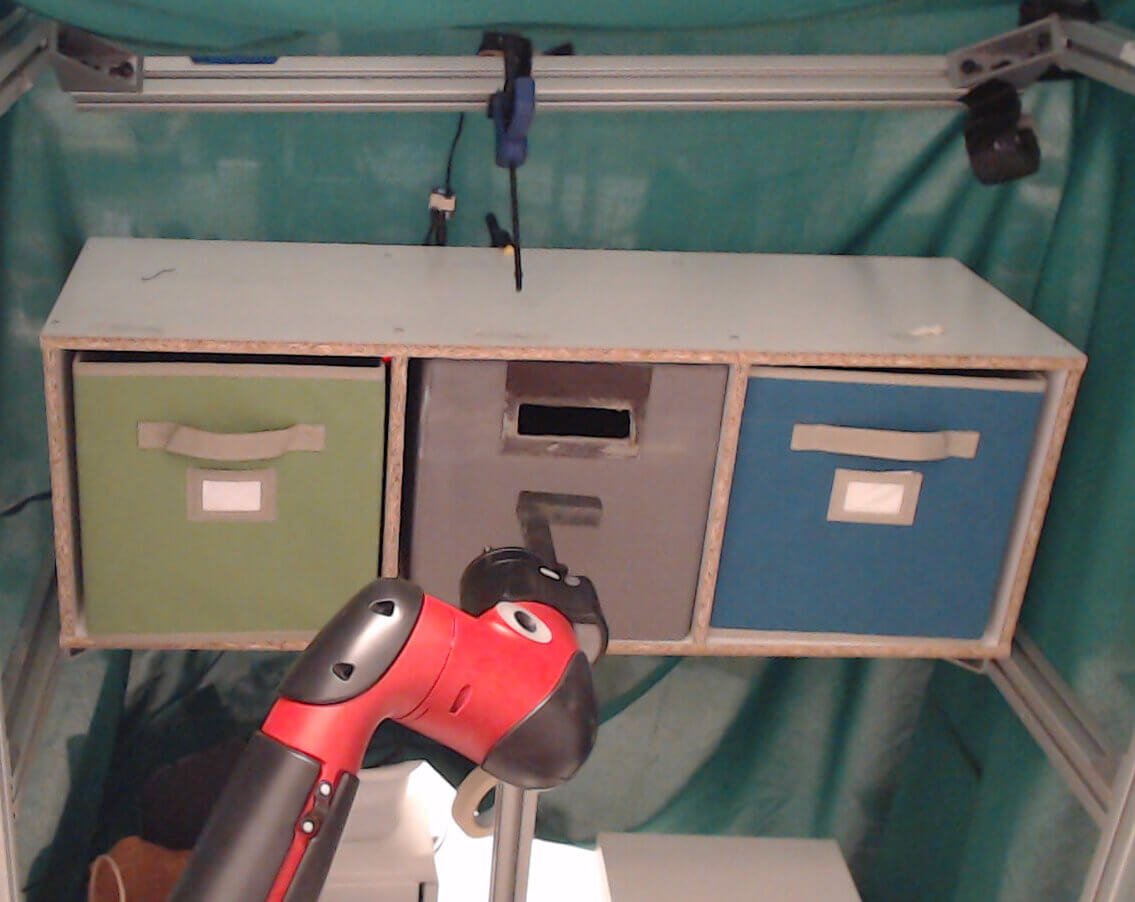
\includegraphics[height=0.6\textwidth]{awac/figures/robot/drawer_img.jpeg}
    \end{subfigure}
    \begin{subfigure}[b]{0.32\textwidth}
        \center
        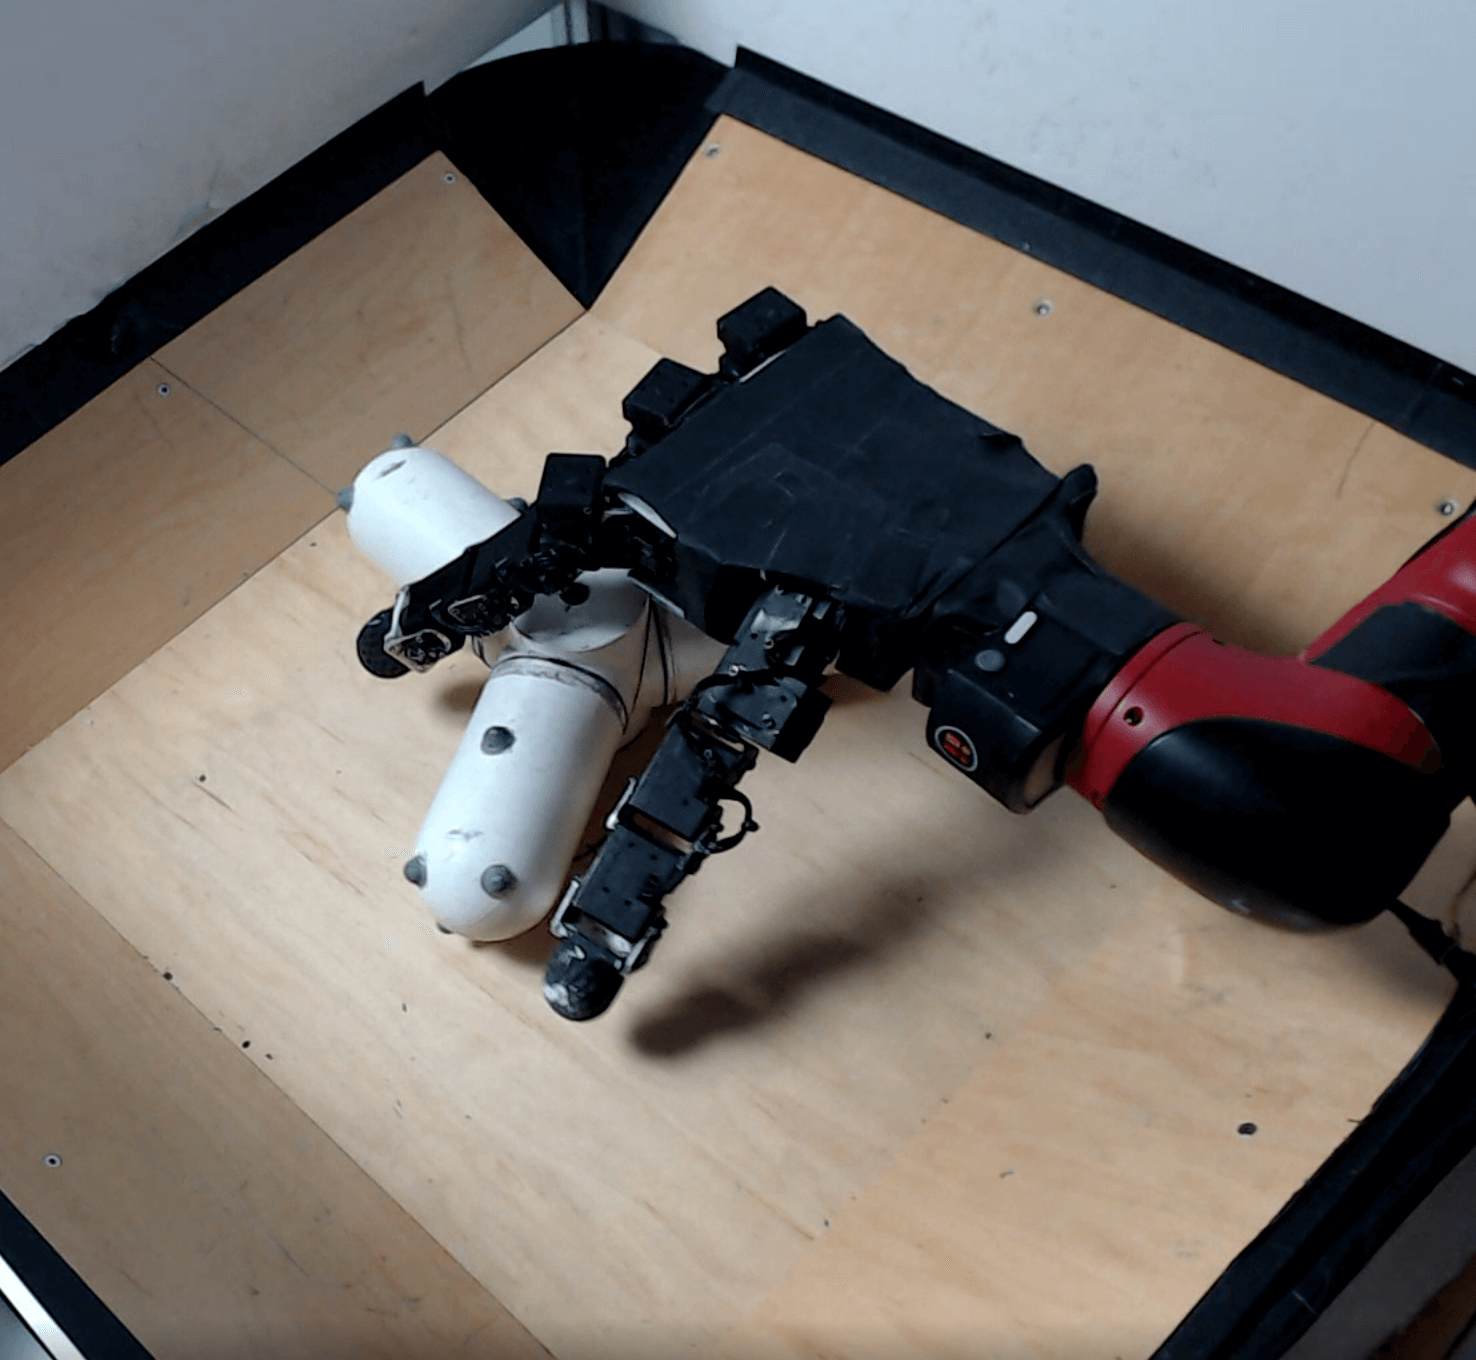
\includegraphics[height=0.6\textwidth]{awac/figures/robot/hand.png}
    \end{subfigure}
    \caption{
    % \footnotesize{
    Full views of the robot hardware setups. Videos are available at \projectpage
    % ABM \cite{siegel2020abm} AWR \cite{peng2019awr} BEAR \cite{kumar19bear} BRAC \cite{wu2019brac} DAPG \cite{rajeswaran2018dextrous} SACfD \cite{vecerik17ddpgfd} SAC+BC \cite{nair2018demonstrations}
    % }
    % \vspace{-0.5cm}
    }
    \label{fig:robot_setups}
\end{figure*}

\pagebreak

\subsection{Hardware Experimental Setup}
\label{sec:hardwaresetup}

Here, we provide further details of the hardware experimental setups, which are pictured in Fig~\ref{fig:robot_setups}.

\noindent \textbf{Dexterous Manipulation with a 3 Fingered Claw.}
\begin{itemize}
    \item State space: 22 dimensions, consisting of joint angles of the robot and rotational position of the object. 
    \item Action space: 9 dimensions, consisting of desired joint angles of the robot.
    \item Reward: $-1$ if the valve is rotated within 0.25 radians of the target, and $0$ otherwise.
    \item Prior data: 10 demonstrations collected by kinesthetic teaching and 200 trajectories of behavior cloned data.
\end{itemize}

\noindent \textbf{Drawer Opening with a Sawyer Arm.}
\begin{itemize}
    \item State space: 4 dimensions, end effector position of the robot and rotational position of the motor attached to the drawer. 
    \item Action space: 3 dimensions, for velocity control of end-effector position.
    \item Reward: $-1$ if the motor is rotated more than 15 radians of the reset position, and $0$ otherwise.
    \item Prior data: 10 demonstrations collected using a 3DConnexion Spacemouse device and 500 trajectories of behavior cloning data.
\end{itemize}

\noindent \textbf{Dexterous Manipulation with a Robotic Hand.}
\begin{itemize}
    \item State space: 25 dimensions, consisting of joint angles of the hand, end effector positions of the arm, object position and target position. 
    \item Action space: 19 dimensions, consisting of desired 16 joint angles of the hand and 3 dimensions for end-effector control of the arm.
    \item Reward: let $o$ be the position of the object, $h$ be the position of the hand, and $g$ be the target location of the object. Then $r = -||o - h|| - 3||o - g||$.
    \item Prior data: 19 demonstrations obtained via kinesthetic teaching and 50 trajectories of behavior cloned data.
\end{itemize}